\documentclass[paper=a4, fontsize=11pt]{scrartcl} % A4 paper and 11pt font size
\usepackage[T1]{fontenc} % Use 8-bit encoding that has 256 glyphs
\usepackage{fourier} % Use the Adobe Utopia font for the document - comment this line to return to the LaTeX default
\usepackage[english]{babel} % English language/hyphenation
\usepackage{amsmath,amsfonts,amsthm} % Math packages
\usepackage{graphicx} % Embedding graphics in document
\usepackage{caption}
\usepackage{listings}
% Custom code listing
\usepackage{color}
\definecolor{codegreen}{rgb}{0,0.6,0}
\definecolor{codegray}{rgb}{0.5,0.5,0.5}
\definecolor{codepurple}{rgb}{0.58,0,0.82}
\definecolor{backcolour}{rgb}{0.95,0.95,0.92}
\lstdefinestyle{mystyle}{
  backgroundcolor=\color{backcolour},
  commentstyle=\color{codegreen},
  keywordstyle=\color{magenta},
  numberstyle=\tiny\color{codegray},
  stringstyle=\color{codepurple},
  basicstyle=\footnotesize,
  breakatwhitespace=false,
  breaklines=true,
  captionpos=b,
  keepspaces=true,
  numbers=left,
  numbersep=5pt,
  showspaces=false,
  showstringspaces=false,
  showtabs=false,
  tabsize=2
}
\lstset{style=mystyle}
% End of custom code listing
\usepackage[utf8]{inputenc}
\usepackage{lipsum} % Used for inserting dummy 'Lorem ipsum' text into the template
\usepackage{sectsty} % Allows customizing section commands
\allsectionsfont{\centering \normalfont\scshape} % Make all sections centered, the default font and small caps
\usepackage{fancyhdr} % Custom headers and footers
\pagestyle{fancyplain} % Makes all pages in the document conform to the custom headers and footers
\fancyhead{} % No page header - if you want one, create it in the same way as the footers below
\fancyfoot[L]{} % Empty left footer
\fancyfoot[C]{} % Empty center footer
\fancyfoot[R]{\thepage} % Page numbering for right footer
\renewcommand{\headrulewidth}{0pt} % Remove header underlines
\renewcommand{\footrulewidth}{0pt} % Remove footer underlines
\setlength{\headheight}{13.6pt} % Customize the height of the header
\numberwithin{equation}{section} % Number equations within sections (i.e. 1.1, 1.2, 2.1, 2.2 instead of 1, 2, 3, 4)
\numberwithin{figure}{section} % Number figures within sections (i.e. 1.1, 1.2, 2.1, 2.2 instead of 1, 2, 3, 4)
\numberwithin{table}{section} % Number tables within sections (i.e. 1.1, 1.2, 2.1, 2.2 instead of 1, 2, 3, 4)
\setlength\parindent{0pt} % Removes all indentation from paragraphs - comment this line for an assignment with lots of text
\theoremstyle{definition}
\newtheorem*{definition}{Definition}
% Theorems
%----------------------------------------------------------------------------------------
% TITLE SECTION
%----------------------------------------------------------------------------------------
\newcommand{\horrule}[1]{\rule{\linewidth}{#1}} % Create horizontal rule command with 1 argument of height
\title{	
  \normalfont \normalsize
  \textsc{University of Oslo} \\ [25pt] % Your university, school and/or department name(s)
  \horrule{0.5pt} \\[0.4cm] % Thin top horizontal rule
  \huge MAT1120 - Assignment 2 \\ % The assignment title
  \horrule{2pt} \\[0.5cm] % Thick bottom horizontal rule
}
\author{Ivar Haugaløkken Stangeby} % Your name
\date{\normalsize\today} % Today's date or a custom date
\begin{document}
\maketitle % Print the title
\section*{Problem 1}
Assume that $U = \left[ \mathbf{u}_1,\dots,\mathbf{u}_n \right]$ is an $\left(n \times n\right)$-matrix.
Verify that $U$ is \textbf{\textit{semi-orthogonal}} if and only if $\mathbf{u}_j \neq \mathbf{0}$ for $j=1,\dots,n$ and all the $\mathbf{u}_j$'s are orthogonal
to each other. In other words, $\mathbf{u}_j \cdot \mathbf{u}_i = 0$ when $j \neq i$.

\begin{definition}
  A quadratic matrix $U$ is called \textbf{semi-orthogonal} if $U^TU$ is a \textbf{diagonal} matrix with only positive entries along the
  main diagonal.
\end{definition}
\begin{definition}
	A matrix $U$ is called \textbf{diagonal} if $U$ has non-zero entries only along the
	main diagonal.
\end{definition}
We now want to show that the condition is both sufficient and neccessary for the matrix to be \textbf{\textit{semi-orthogonal}}.

Let us first form the matrix $B = U^TU$.
\begin{align*}
  B = \begin{pmatrix}
	\mathbf{u}_1 \\
	\vdots \\
	\mathbf{u}_n\\
  \end{pmatrix} \begin{bmatrix}
	\mathbf{u}_1 & \hdots & \mathbf{u}_n\\
  \end{bmatrix} = \begin{bmatrix}
	\mathbf{u}_1 \cdot \mathbf{u}_1 & \hdots & \mathbf{u}_1\cdot\mathbf{u}_n \\
	\vdots & \ddots & \vdots \\
	\mathbf{u}_n \cdot \mathbf{u}_1 & \hdots & \mathbf{u}_n\cdot\mathbf{u}_n\\
  \end{bmatrix}.
\end{align*}
Assume now that each column in $U$ is orthogonal to all the other columns. We can then directly see that all the entries in $B$ that are not
along the main diagonal must be zero. It is now sufficient to show that the entries along the main diagonal must be strictly positive.
Let $\mathbf{u} \in U$ be an arbitrary vector from $U$.
\begin{align*}
  \mathbf{u}\cdot\mathbf{u} = u_1^2 + \dots + u_n^2.
\end{align*}
Each term is squared, thus $\mathbf{u}\cdot\mathbf{u}$ is strictly positive.

If we instead were to assume that each column in $U$ was \textbf{not} orthogonal to the other columns, we can directly from the matrix $B$ see that we get
non-zero entries that are not along the main diagonal, which contradict the condition that $B$ must be a diagonal matrix.
We can then conclude that $U$ is \textbf{\textit{semi-orthogonal}} if and only if the columns of $U$ are orthogonal, and not the zero vector.

Further assume that $U$ is \textbf{\textit{semi-orthogonal}} and let
\begin{align*}
  \mathbf{u}_j' = \frac{1}{\mathbf{u}_j\cdot\mathbf{u}_j}\mathbf{u}_j, \qquad j = 1,\dots,n.
\end{align*}
Argue that $U$ is invertible and that
\begin{align*}
  U^{-1} = \left[ \mathbf{u}_1' \dots \mathbf{u}_n' \right]^T.
\end{align*}
Let us look at the columns of $U, \left\{ \mathbf{u}_1,\dots,\mathbf{u}_n \right\}$.
If the set of columns is an orthogonal set of non-zero vectors then the set is linearly independent.
Since we assumed that $U$ is \textit{\textbf{semi-orthogonal}}, then it follows that the set of columns is linearly independent.\\
By the \underline{Invertible Matrix Theorem}, $U$ is invertible.

We now want to show that the inverse of $U$ is as given above.
Let us check if $UU^{-1} = I$.
\begin{align*}
  UU^{-1} = \begin{bmatrix}
	\mathbf{u}_1 & \hdots & \mathbf{u}_n
  \end{bmatrix} \begin{pmatrix}
	\mathbf{u}_1'\\
	\vdots\\
	\mathbf{u}_n'\\
  \end{pmatrix} = \begin{bmatrix}
	\mathbf{u}_1\cdot\mathbf{u}_1' & \hdots & \mathbf{u}_1\cdot\mathbf{u}_n'\\
	\vdots & \ddots & \vdots \\
	\mathbf{u}_n\cdot\mathbf{u}_1' & \hdots & \mathbf{u}_n\cdot\mathbf{u}_n'\\
  \end{bmatrix}
\end{align*}
Let $\mathbf{x}, \mathbf{y}' \in \left\{ \mathbf{u}_1, \dots, \mathbf{u}_n \right\}$.\\
\begin{itemize}
  \item $\mathbf{x} = \mathbf{y} \Rightarrow \mathbf{x}\cdot\mathbf{y}' = 1$
  \item $\mathbf{x} \neq \mathbf{y} \Rightarrow \mathbf{x}\cdot\mathbf{y}' = 0$
\end{itemize}
We have that $\mathbf{x} = \mathbf{y}$ only along the main diagonal, therefore $UU^{-1} = I$.

\section*{Problem 2}
Divide $\left[ 0, \pi \right]$ into 3 intervals of length $\frac{\pi}{3}$ and let $t_1, t_2$ and $t_3$ be the midpoints of these intervals.
Let
\begin{align*}
  % 3x3
C_3 =  
  \begin{bmatrix}
   1 & \cos (t_1) & \cos (2t_1) \\
   1 & \cos (t_2) & \cos (2t_2) \\
   1 & \cos (t_3) & \cos (2t_3) \\
  \end{bmatrix} & \qquad S_3 = 
  \begin{bmatrix}
   \sin (t_1) & \sin (2t_1) & \sin (3t_1) \\
   \sin (t_2) & \sin (2t_2) & \sin (3t_2) \\
   \sin (t_3) & \sin (2t_3) & \sin (3t_3) \\
  \end{bmatrix}
\end{align*}
Plugging in the values of $t_1, t_2$ and $t_3$ gives: 
\begin{align*}
  C_3 = 
  \begin{bmatrix}
  1 & \frac{\sqrt{3}}{2} & \frac{1}{2}\\
  1 & 0 & -1 \\
  1 & -\frac{\sqrt{3}}{2} & \frac{1}{2} \\
\end{bmatrix} & \qquad S_3 = 
\begin{bmatrix}
  \frac{1}{2} & \frac{\sqrt{3}}{2} & 1 \\
  1 & 0 & -1 \\
  \frac{1}{2} & -\frac{\sqrt{3}}{2} & 1\\
\end{bmatrix}
\end{align*}

These two matrices are \textit{\textbf{semi-orthogonal}} because $C_3^TC_3$ and $S_3^TS_3$ are diagonal matrices with only positive entries along the main diagonal.
\begin{align*}
  C_3^TC_3 = \begin{bmatrix}
	3 & 0 & 0 \\
	0 & \frac{3}{2} & 0 \\
	0 & 0 & \frac{3}{2}\\
  \end{bmatrix} \qquad S_3^TS_3 =
  \begin{bmatrix}
	\frac{3}{2} & 0 & 0 \\
	0 & \frac{3}{2} & 0 \\
	0 & 0 & 3\\
  \end{bmatrix}
\end{align*}
Based on this we know that the inverses of these matrices are given by $U^{-1} = \begin{bmatrix}
  \mathbf{u}_1' & \dots & \mathbf{u}_n'
\end{bmatrix}^T$
This gives us the inverses:
\begin{align*}
  C_3^{-1} = 
 \begin{bmatrix}
   \frac{1}{3} & \frac{1}{3} & \frac{1}{3} \\
   \frac{\sqrt{3}}{3} & 0 &  -\frac{\sqrt{3}}{3} \\
   \frac{1}{3} & -\frac{2}{3} & \frac{1}{3}\\
 \end{bmatrix} \qquad & S_3^{-1} = 
 \begin{bmatrix}
   \frac{1}{3} & \frac{2}{3} & \frac{1}{3}\\
   \frac{\sqrt{3}}{3} & 0 & -\frac{\sqrt{3}}{3}\\
   \frac{1}{3} & -\frac{1}{3} & \frac{1}{3}\\
 \end{bmatrix}
\end{align*}

\section*{Problem 3}
According to my python program both the matrices $C$ and $S$ are \textit{\textbf{semi-orthogonal}}, with the following inverses:
\begin{align*}
  C^{-1} = \input{../src/C_matrix.tex}\\
  \\
  S^{-1} = \input{../src/S_matrix.tex}
\end{align*}
Multiplying the matrices with the respective inverses yields the identity matrix in both cases.

\section*{Problem 4}
Let $\mathcal{F}([0, 2\pi], \mathbb{R})$ be the vector space consisting of all real functions defined on $\left[ 0, \pi \right]$ and let
$\mathcal{W}_c$ be its subspace that is spanned by the set
\begin{align*}
  \mathcal{C} = \left\{ 1, \cos(t), \cos(2t), \dots, \cos(7t) \right\}
\end{align*}
We showed in the previous problem that $C$ is semi-orthogonal. It then follows that $C$ is invertible, which means that the columns of $C$ neccessarily
has to be linearly independent. This, in turn, means that $\mathcal{C}$ is a basis for $\mathcal{W}_C$.
There is a result regarding signal spaces that tells ut that it is sufficient to show that this holds for the discrete values
$t = t_1, \dots, t_8$

\section*{Problem 5}
Let $T_c : \mathcal{W}_c \rightarrow \mathbb{R}^8$ be defined by:
$$ T_c\left( h \right) = \left( h(t_1),\dots,h(t_8) \right) $$
for $h \in \mathcal{W}_c$, and let $\epsilon = \left\{ \mathbf{e}_1, \dots, \mathbf{e}_8 \right\}$. \\

Verify that $C$ is the matrix of $T_c$ with respect to the bases $\mathcal{C}$ and $\epsilon$, and show that $T_c$ is an isomorphism. 

$C$ is a matrix with those properties if $T_c(\mathbf{x})$ maps $\left[\mathbf{x}\right]_\mathcal{C}$ to $\left[ T_c(\mathbf{x}) \right]_\epsilon$.

Let $h$ be any arbitrary vector in $\mathcal{W}_c$ with respect to the basis $\mathcal{C}$
\begin{align*}
  h = \begin{bmatrix}
    \lambda_1 \\
	\vdots \\
	\lambda_8\\
  \end{bmatrix}
\end{align*}.

Multiplying from the left by the matrix $C$, we get
\begin{align*}
  Ch = \begin{bmatrix}
   1 & \dots & \cos(7t_1)\\
   \vdots & \dots & \vdots \\
   1 & \dots & \cos(7t_8)\\
  \end{bmatrix} \begin{bmatrix}
	\lambda_1\\
	\vdots \\
	\lambda_8\\
  \end{bmatrix} = \left[\left( h(t_1), \dots, h(t_8) \right)\right]_\epsilon
\end{align*}
Since $h$ was any arbitrary vector from $\mathcal{W}_c$, this means that $C$ is the matrix of $T_c$ with respect to the bases $\mathcal{C}$ and $\epsilon$.

Since $\mathcal{C}$ is a basis for $\mathcal{W}_c$, and $\epsilon$ is a basis for $\mathbb{R}^8$ it follows that $T_c$ is a bijective transformation. Since $T_c$ is linear, this 
means $T_c$ is an isomorph transformation. 
The matrix for $T_c^{-1}$ is $C^{-1}$. 
\section*{Problem 6}
Let $g \in \mathcal{F}\left( \left[ 0, \pi \right], \mathbb{R} \right)$ and set
$\mathbf{y} = \left(g(t_1), \dots, g(t_8)\right) \in \mathbb{R}^8$. In addition, let
\begin{align*}
  g^c = T_c^{-1}(\mathbf{y}) \in \mathcal{W}_c
\end{align*}

Show that $g^c$ is an 8-midpoint interpolation of $g$ on the interval $\left[ 0, \pi \right]$ that satisfy $\left[ g^c \right]_C = C^{-1}\mathbf{y}$.

$g^c$ is a function in $\mathcal{W}_c$ that is defined in such a way that $g^c$ interpolate $g$ in the midpoints $t_1, \dots, t_8$. This means that $g^c$ is an 8-midpoint interpolation of $g$ on $\left[ 0, \pi \right]$ since, 

\begin{align*}
  Cg^c &= CT_c^{-1}(\mathbf{y}) = CC^{-1}\mathbf{y} = \mathbf{y}\\
  T_c(g^c) &= C\left[ g^c \right]_C = y \Leftrightarrow \left[ g^c \right]_C = C^{-1}\mathbf{y}
\end{align*}.

\section*{Problem 7}

Argue that $V_l$ and $V_o$ are subspaces of $V$. 

We want to show that both $V_l$ and $V_o$ are closed under addition, multiplication by a
scalar, and also that the zero-function is both spaces. 
Ill show the calculations for $V_l$, the same is proved for $V_o$ similarly.
Let $f_1, f_2 \in V_l$, and set $f_3 = f_1 + f_2$.
We now want to show that $f_3 \in V_l$.
\begin{align*}
f_3(-t) = (f_1 + f_2)(-t) = f_1(-t) + f_2(-t) = f_1(t) = f_2(t) = f_3(t)
\end{align*}
Thus $V_l$ is closed under addition.
Now, let $f_3 = cf_1, c \in \mathbb{R}$.
We want to show that $f_3 \in V_l$
\begin{align*}
  f_3(-t) =(cf_1)(t) =  cf_1(-t) = cf_1(t) = f_3(t) \in V_l.\\
\end{align*}.

We now want to show that if $f \in V$, then $f_l \in V_l$ and $f_o \in V_o$ as well as $f = f_l + f_o$.

Assume $f \in V$. We then have:
\begin{align*}
  f_l = \frac{1}{2}\left( f + T\left( f \right) \right) \\
  f_o = \frac{1}{2}\left( f - T(f) \right)\\
  f_l + f_o = \frac{1}{2}2f = f\\
\end{align*}
To show $f_l \in V_l$ and $f_o \in V_o$.
\begin{align*}
  \left[ T(f_l) \right](t) &= \frac{1}{2}\left( \left[ T(f) \right](t) + \left[ T(T(f)) \right](t) \right)\\
  &= \frac{1}{2}\left( f(t) + f(-t) \right) = f_l(t)
\end{align*}
Thus $f_l \in V_l$.
\begin{align*}
  \left[ T(f_o) \right](t) &= \frac{1}{2}(f(-t) - f(t)) \\
  &= f_o(-t) = -f_o(t).
\end{align*}
Thus $f_o \in V_o$.

\pagebreak
\section*{Problem 8}
This is a 16-midpoint interpolation of the function $f(t) = \left(\pi^2 - t^2\right)e^{t/2\pi}, t \in \left[ -\pi, \pi \right]$
\begin{figure}[!h]
	\centering
	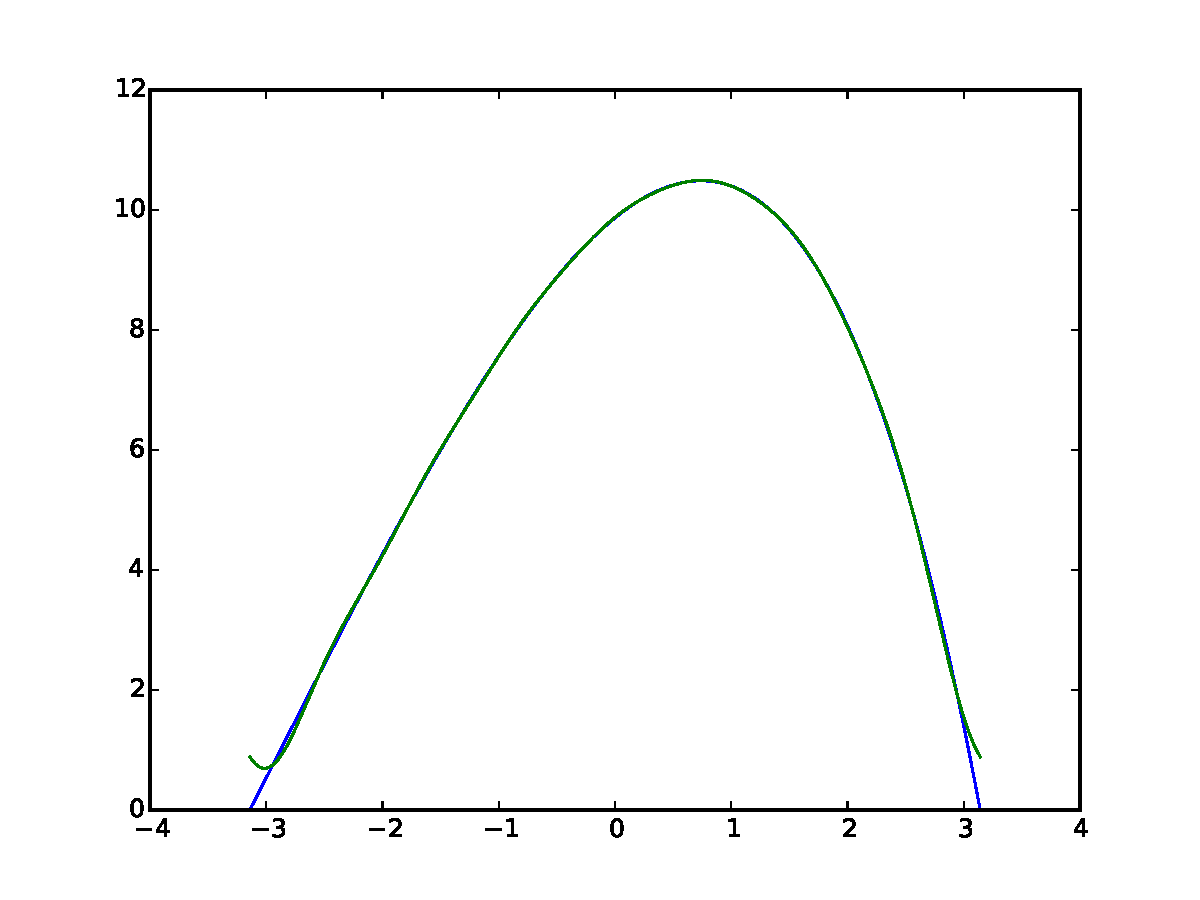
\includegraphics[scale=0.5]{Problem8}
\end{figure}
\section*{Problem 9}
This is a 16-midpoint interpolation of the function $f(t) = te^{t/2\pi}, t \in \left[ -\pi, \pi \right]$
\begin{figure}[!h]
	\centering
	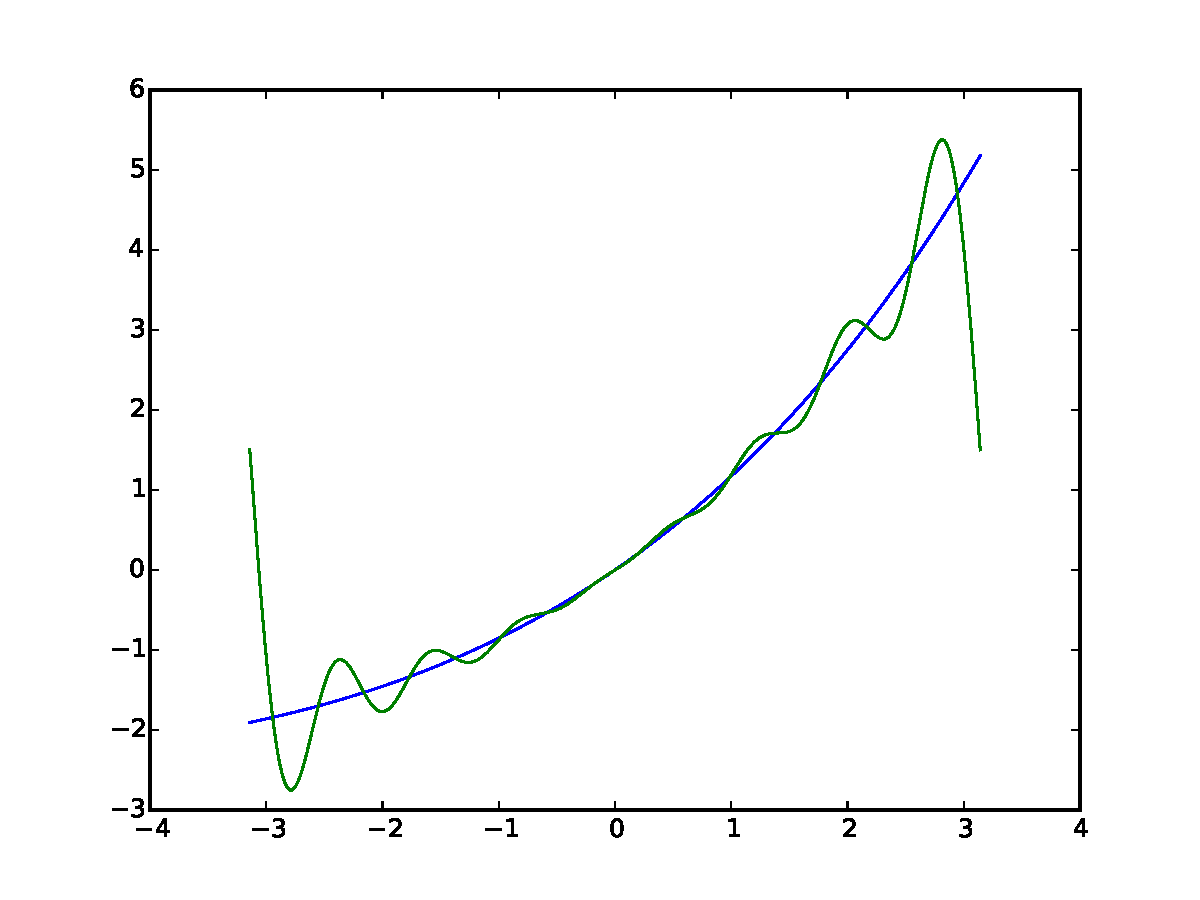
\includegraphics[scale=0.5]{Problem9}
\end{figure}
\pagebreak

\section*{Appendix}
\lstinputlisting{../src/assignment.py}
\pagebreak
\lstinputlisting{../src/problem3.py}
\pagebreak
\lstinputlisting{../src/problem8.py}
\end{document}
